\section{Option Strategies}
\label{sect:option-strat}
\begin{enumerate}
\item In this section, we use the ``basic'' option positions: long call (LC),
long put (LP), short call (SC), and short put (SP), to ``compose'' more complex
option strategies.
\end{enumerate}
\subsection{Floors}
\begin{enumerate}
\item A \emph{floor} is a strategy that insures a long position in an asset
\faIcon{apple-alt}.
\item P/L (at time \(T\)) graph for long \faIcon{apple-alt}:
\begin{center}
\begin{tikzpicture}[]
\begin{axis}[domain=0:5, ymin=-2.5, ymax=2.5, xmax=5.5, axis y line=left, axis x line=middle,
xtick={2.2}, ytick={-2.2}, title={Long \faIcon{apple-alt}},
xticklabel={\(S_0e^{rT}\)}, xticklabel style={xshift=0.3cm},
yticklabel={\(-S_0e^{rT}\)},
ylabel=P/L,
ylabel style={at={(axis description cs:0,1)}, anchor=south, rotate=-90},
xlabel=\(S_T\),
xlabel style={anchor=west}
]
\addplot[blue, thick]{x-2.2};
\node[red] at (1.5,-1.5) {risk \faIcon{exclamation-triangle}};
\draw[opacity=0.5, red, line width=0.2cm, line cap=round] (0,-2.2) -- (2.1,-0.1);
\end{axis}
\end{tikzpicture}
\end{center}
There is a risk for long \faIcon{apple-alt}: If the price of \faIcon{apple-alt}
drops \faIcon{chart-area} significantly after \(T\) years, we would suffer a
great loss.

\item To hedge (reduce) this risk \faIcon{shield-alt}, we can long a put on
\faIcon{apple-alt} since the ``initial positive'' part of the P/L graph for LP
can help reducing the risk:
\begin{center}
\begin{tikzpicture}[declare function={func(\x) = (\x <= 2) * (1.5-x) + (\x > 2) * -0.5;}]
\begin{axis}[domain=0:5, ymin=-2.5, ymax=2.5, xmax=5.5, axis y line=left, axis x line=middle,
xtick=\empty, ytick=\empty, samples=100,
ylabel=P/L,
ylabel style={at={(axis description cs:0,1)}, anchor=south, rotate=-90},
xlabel=\(S_T\),
xlabel style={anchor=west}, samples=100,
title=LP
]
\addplot[blue, thick]{func(x)};
\draw[opacity=0.4, ForestGreen, line width=0.2cm, line cap=round, line join=round] (0,1.5) -- (1.4,0.1);
\end{axis}
\end{tikzpicture}
\end{center}
This forms a \defn{floor} (long \faIcon{apple-alt} and LP):
\begin{center}
\begin{tikzpicture}[
declare function={
lp(\x) = (\x <= 2) * (1.5-x) + (\x > 2) * -0.5;
la(\x) = (x-2.2);
}
]
\begin{axis}[domain=0:5, ymin=-2.5, ymax=2.5, xmax=5.5, axis y line=left, axis x line=middle,
title={{\color{violet}Floor} = {\color{blue}Long \faIcon{apple-alt}} + {\color{orange}LP}},
xtick={2.2}, xticklabel={\(S_0e^{rT}\)}, xticklabel style={yshift=0.7cm, xshift=0.2cm},
ytick={-2.2},
yticklabel={\(-S_0e^{rT}\)},
ylabel=P/L,
ylabel style={at={(axis description cs:0,1)}, anchor=south, rotate=-90},
xlabel=\(S_T\),
xlabel style={anchor=west}, samples=100
]
\addplot[blue, thick, dashed, opacity=0.5]{la(x)};
\addplot[orange, thick, dashed, opacity=0.5]{lp(x)};
\addplot[violet, thick]{la(x)+lp(x)};
\draw[opacity=0.4, ForestGreen, line width=0.2cm, line cap=round, line join=round] (0,-0.7) -- (2,-0.7) -- (2.6,-0.1);
\node[ForestGreen] at (1.2,-0.4) {hedged \faIcon{shield-alt} risk};
\draw[-Latex] (3,-1) to[bend left] (1,-0.8);
\node[] () at (3.5,-0.8) {``Floor''};
\node[violet] () at (4,0.3) {slope = 1};
\end{axis}
\end{tikzpicture}
\end{center}
\item The P/L (at time \(T\)) of the floor is given by
\[
\underbrace{S_T-S_0e^{rT}}_{\text{long \faIcon{apple-alt}}} +
\underbrace{(K-S_T)_{+}-P_0e^{rT}}_{\text{LP}}
=S_T+(K-S_T)_{+}-(S_0+P_0)e^{rT}.
\]
\item Based on the P/L of the floor and the no-arbitrage principle, it turns
out that we can derive a bound on the put option price \(P_0\). Consider the
payoff graph:
\begin{center}
\begin{tikzpicture}[
declare function={
lp(\x) = (\x <= 2) * (2-x) + (\x > 2) * 0;
la(\x) = (x);
}
]
\begin{axis}[domain=0:5, ymin=-2.5, xmax=5.5, axis y line=left, axis x line=middle,
xtick={2}, title={{\color{violet}Floor} = {\color{blue}Long \faIcon{apple-alt}} + {\color{orange}LP}},
xticklabel={\(K\)},
ytick={2},
yticklabel={\(K\)}, ylabel=Payoff, ylabel style={at={(axis description cs:0,1)}, anchor=south, rotate=-90},
xlabel=\(S_T\),
xlabel style={anchor=west}, samples=100
]
\addplot[blue, thick, dashed, opacity=0.5]{la(x)};
\addplot[orange, thick, dashed, opacity=0.5]{lp(x)};
\addplot[violet, thick]{la(x)+lp(x)};
\node[violet] () at (4,2.5) {slope = 1};
\end{axis}
\end{tikzpicture}
\end{center}
\begin{note}
The payoff of the floor is \(S_T+(K-S_T)_{+}\).
\end{note}

\item \label{it:put-price-lb}
Let \(\pi_0\) be the time-0 price of the floor (which is \(S_0+P_0\)). Then,
its P/L can be expressed as
\[
S_T+(K-S_T)_{+}-\pi_0 e^{rT}.  \]
Since \(\pi_0 e^{rT}>0\) is a constant with respect to \(S_T\), the P/L graph
can also be obtained by shifting the payoff graph \emph{downward} by
\(\pi_0e^{rT}\):
\begin{center}
\begin{tikzpicture}[
declare function={
lp(\x) = (\x <= 2) * (2-x) + (\x > 2) * 0;
la(\x) = (x);
}
]
\begin{axis}[domain=0:5, ymin=-2.5, xmax=5.5, axis y line=left, axis x line=middle,
xtick={2}, title={{\color{violet}Floor} = Long \faIcon{apple-alt} + LP},
xticklabel={\(K\)},
ytick={2,-0.7},
yticklabels={\(K\),\(K-\pi_0e^{rT}\)}, ylabel=P/L, ylabel style={at={(axis description cs:0,1)}, anchor=south, rotate=-90},
xlabel=\(S_T\),
xlabel style={anchor=west}, samples=100
]
\addplot[violet, thick, dashed, opacity=0.3]{lp(x)+la(x)};
\addplot[violet, thick]{lp(x)+la(x)-2.7};
\draw[-Latex, brown] (0.8,1.8) -- (0.8,-0.5);
\draw[-Latex, brown] (1.6,1.8) -- (1.6,-0.5);
\draw[-Latex, brown] (2.4,2.2) -- (2.4,-0.1);
\draw[-Latex, brown] (3.2,3) -- (3.2,0.7);
\draw[-Latex, brown] (4,3.8) -- (4,1.5);
\node[brown] () at (4.8,3.3) {\(-\pi_0e^{rT}\)};
\node[violet] () at (4,0.3) {slope = 1};
\end{axis}
\end{tikzpicture}
\end{center}
Under the no-arbitrage principle, the P/L cannot be always nonnegative. Hence,
we must have
\[
K-(S_0+P_0)e^{rT}<0 \implies P_0>Ke^{-rT}-S_0,
\]
yielding a lower bound of the put option price \(P_0\).
\item From the payoff and P/L graphs of the floor, one can also observe that its
``shape'' is similar to the respective graphs for \emph{long call}:
\begin{center}
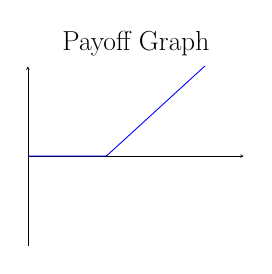
\begin{tikzpicture}[scale=0.4, declare function={func(\x) = (\x <= 2) * 0 + (\x > 2) * (x-2);}]
\begin{axis}[domain=0:5, ymin=-2.5, ymax=2.5, xmax=5.5, axis y line=left, axis x line=middle,
xtick=\empty, ytick=\empty, samples=100, title=\Huge{Payoff Graph}]
\addplot[blue, thick]{func(x)};
\end{axis}
\end{tikzpicture}
\qquad
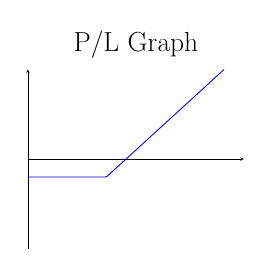
\begin{tikzpicture}[scale=0.4, declare function={func(\x) = (\x <= 2) * -0.5 + (\x > 2) * (x-2.5);}]
\begin{axis}[domain=0:5, ymin=-2.5, ymax=2.5, xmax=5.5, axis y line=left, axis x line=middle,
xtick=\empty, ytick=\empty, samples=100, title=\Huge{P/L Graph}]
\addplot[blue, thick]{func(x)};
\end{axis}
\end{tikzpicture}
\end{center}

\item We can observe that the payoff graph of the floor can be obtained by
shifting the payoff graph of long call \emph{upward} by \(K\).

Indeed, the floor can also be ``composed'' using a \emph{long call} on
\faIcon{apple-alt} and a loan (lending \faIcon{dollar-sign} risk-free at time
0 such that a cash flow of \(K\) can be collected at time \(T\)).

\begin{note}
Sometimes the act of lending/borrowing \faIcon{dollar-sign} (risk-free) is
described as \emph{buying}/\emph{selling} a (risk-free) bond \faIcon{scroll}
\faIcon{arrow-right} having a \emph{long}/\emph{short} position in bond
\faIcon{scroll}.

The amount paid when buying the bond \faIcon{scroll} is the amount \emph{lent}
to the seller (borrower). Then, \faIcon{scroll} entitles its owner to later
collect proceeds from the bond seller.
\end{note}

To be more precise, we can ``decompose'' the payoff graph like below:

\begin{center}
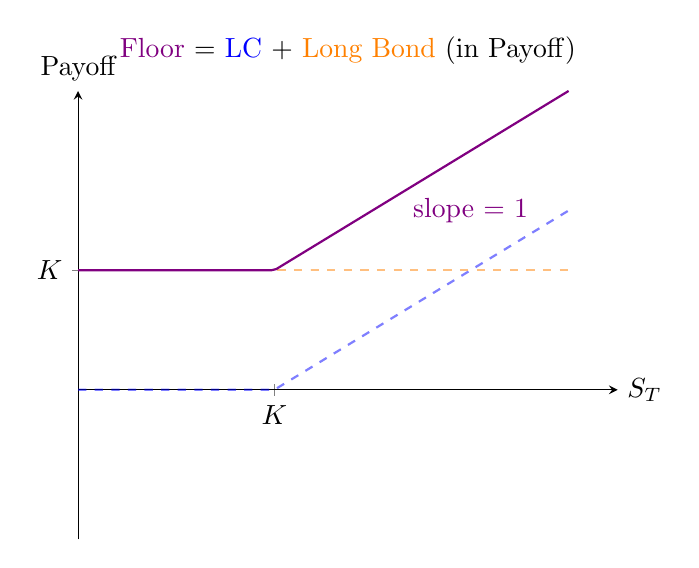
\begin{tikzpicture}[
declare function={
lc(\x) = (\x <= 2) * 0 + (\x > 2) * (\x - 2);
lb(\x) = 2;
}
]
\begin{axis}[domain=0:5, ymin=-2.5, xmax=5.5, axis y line=left, axis x line=middle,
xtick={2}, title={{\color{violet}Floor} = {\color{blue}LC} + {\color{orange}Long Bond} (in Payoff)},
xticklabel={\(K\)},
ytick={2},
yticklabel={\(K\)}, ylabel=Payoff, ylabel style={at={(axis description cs:0,1)}, anchor=south, rotate=-90},
xlabel=\(S_T\),
xlabel style={anchor=west}, samples=100
]
\addplot[blue, thick, dashed, opacity=0.5]{lc(x)};
\addplot[orange, thick, dashed, opacity=0.5]{lb(x)};
\addplot[violet, thick]{lb(x)+lc(x)};
\node[violet] () at (4,3) {slope = 1};
\end{axis}
\end{tikzpicture}
\end{center}
Algebraically we can write
\[
\underbrace{S_T+(K-S_T)_{+}}_{\text{floor payoff}}
=\underbrace{K+(S_T-K)_{+}}_{\mathclap{\text{``LC + long bond'' payoff}}},
\]
Since floor and ``LC + long bond'' have the same payoff, by the law of one
price, their (time-0) prices must be the same. (This is useful for deriving the
\emph{put-call parity}; See \cref{subsect:put-call-parity}.)
\end{enumerate}
\subsection{Caps}
\begin{enumerate}
\item A \emph{cap} is a strategy that insures a short position in an asset \faIcon{apple-alt}.

\item P/L (at time \(T\)) graph for short \faIcon{apple-alt}:
\begin{center}
\begin{tikzpicture}[]
\begin{axis}[domain=0:5, ymin=-2.5, ymax=2.5, xmax=5.5, axis y line=left, axis x line=middle,
xtick={2.2}, ytick={2.2}, title={Short \faIcon{apple-alt}},
xticklabel={\(S_0e^{rT}\)}, xticklabel style={xshift=0.5cm, yshift=0.6cm},
yticklabel={\(S_0e^{rT}\)},
ylabel=P/L,
ylabel style={at={(axis description cs:0,1)}, anchor=south, rotate=-90},
xlabel=\(S_T\),
xlabel style={anchor=west}
]
\addplot[blue, thick]{2.2-x};
\node[red] at (4,-0.7) {risk \faIcon{exclamation-triangle}};
\draw[opacity=0.5, red, line width=0.2cm, line cap=round] (2.3,-0.1) -- (4.7,-2.5);
\end{axis}
\end{tikzpicture}
\end{center}
There is a risk for short \faIcon{apple-alt}: If the price of
\faIcon{apple-alt} rises \faIcon{chart-line} significantly after \(T\) years,
we would suffer a great loss.

\item To hedge this risk \faIcon{shield-alt}, we can long a call on
\faIcon{apple-alt} since the ``later positive'' part of the P/L graph for LC
can help reducing the risk:
\begin{center}
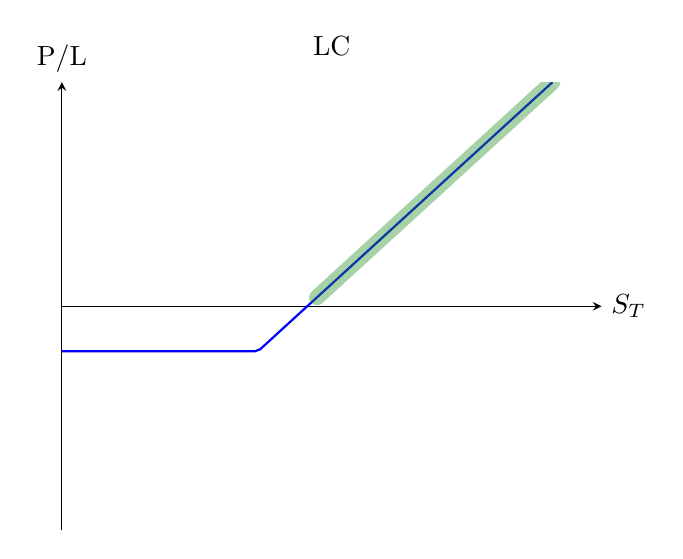
\begin{tikzpicture}[declare function={func(\x) = (\x <= 2) * (-0.5) + (\x > 2) * (\x-2.5);}]
\begin{axis}[domain=0:5, ymin=-2.5, ymax=2.5, xmax=5.5, axis y line=left, axis x line=middle,
xtick=\empty, ytick=\empty, samples=100,
ylabel=P/L,
ylabel style={at={(axis description cs:0,1)}, anchor=south, rotate=-90},
xlabel=\(S_T\),
xlabel style={anchor=west}, samples=100,
title=LC
]
\addplot[blue, thick]{func(x)};
\draw[opacity=0.4, ForestGreen, line width=0.2cm, line cap=round, line join=round] (2.6,0.1) -- (5,2.5);
\end{axis}
\end{tikzpicture}
\end{center}


This forms a \defn{cap} (short \faIcon{apple-alt} and LC):
\begin{center}
\begin{tikzpicture}[
declare function={
lc(\x) = (\x <= 2) * -0.5 + (\x > 2) * (\x-2.5);
sa(\x) = (2.2-\x);
}
]
\begin{axis}[domain=0:5, ymin=-2.5, ymax=2.5, xmax=5.5, axis y line=left, axis x line=middle,
title={{\color{violet}Cap} = {\color{blue}Short \faIcon{apple-alt}} + {\color{orange}LC}},
xtick={2.2}, xticklabel={\(S_0e^{rT}\)}, xticklabel style={yshift=0.6cm, xshift=0.5cm},
ytick={2.2},
yticklabel={\(S_0e^{rT}\)},
ylabel=P/L,
ylabel style={at={(axis description cs:0,1)}, anchor=south, rotate=-90},
xlabel=\(S_T\),
xlabel style={anchor=west}, samples=100
]
\addplot[blue, thick, dashed, opacity=0.5]{sa(x)};
\addplot[orange, thick, dashed, opacity=0.5]{lc(x)};
\addplot[violet, thick]{sa(x)+lc(x)};
\draw[opacity=0.4, ForestGreen, line width=0.2cm, line cap=round, line join=round] (1.8,-0.1) -- (2,-0.3) -- (5,-0.3);
\draw[-Latex] (3,-1.5) to[bend right] (4,-0.6);
\node[text width=4cm] () at (2,-1.5) {``Cap'' (cannot ``go down'' further)};
\node[violet] () at (2,0.7) {slope = \(-1\)};
\node[ForestGreen] at (2.8,-0.6) {hedged \faIcon{shield-alt} risk};
\end{axis}
\end{tikzpicture}
\end{center}
\item The P/L (at time \(T\)) of the cap is given by
\[
\underbrace{-S_T+S_0e^{rT}}_{\text{long \faIcon{apple-alt}}} +
\underbrace{(S_T-K)_{+}-C_0e^{rT}}_{\text{LC}}
=-S_T+(S_T-K)_{+}-(-S_0+C_0)e^{rT}.
\]
\item Similarly, based on the P/L of the cap and the no-arbitrage principle, we
can bound the call option price \(C_0\).  Consider the \emph{payoff}
graph:
\begin{center}
\begin{tikzpicture}[
declare function={
lc(\x) = (\x <= 2) * 0 + (\x > 2) * (\x-2);
sa(\x) = (-\x);
}
]
\begin{axis}[domain=0:5, ymin=-2.5, xmax=5.5, axis y line=left, axis x line=middle,
xtick={2}, title={{\color{violet}Cap} = {\color{blue}Short \faIcon{apple-alt}} + {\color{orange}LC}},
xticklabel={\(K\)},
ytick={-2},
yticklabel={\(-K\)}, ylabel=Payoff, ylabel style={at={(axis description cs:0,1)}, anchor=south, rotate=-90},
xlabel=\(S_T\),
xlabel style={anchor=west}, samples=100
]
\addplot[blue, thick, dashed, opacity=0.5]{sa(x)};
\addplot[orange, thick, dashed, opacity=0.5]{lc(x)};
\addplot[violet, thick]{sa(x)+lc(x)};
\node[violet] () at (2,-1) {slope = \(-1\)};
\end{axis}
\end{tikzpicture}
\end{center}
\begin{note}
The payoff of the cap is \(-S_T+(S_T-K)_{+}\).
\end{note}

\item \label{it:call-price-ub}
Let \(\pi_0\) be the time-0 price of the cap (which is \(-S_0+C_0\)). Then,
its P/L can be expressed as
\[
-S_T+(S_T-K)_{+}-\pi_0e^{rT}.
\]
Under the no-arbitrage principle, the P/L cannot be always nonpositive.
(Otherwise, \emph{reverse} cap would have an always nonnegative P/L
\faIcon{arrow-right} arbitrage!) Consequently, we need to shift the payoff
graph \emph{upward} to get the P/L graph. Hence, we have
\[
\pi_0<0\implies C_0<S_0,
\]
yielding an upper bound of the call option price \(C_0\).

\item Again, from the payoff and P/L graphs of the cap, one can observe
that its ``shape'' is similar to the respective graphs for \emph{long put}:
\begin{center}
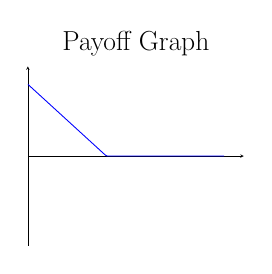
\begin{tikzpicture}[scale=0.4, declare function={func(\x) = (\x <= 2) * (2-\x) + (\x > 2) * 0;}]
\begin{axis}[domain=0:5, ymin=-2.5, ymax=2.5, xmax=5.5, axis y line=left, axis x line=middle,
xtick=\empty, ytick=\empty, samples=100, title=\Huge{Payoff Graph}]
\addplot[blue, thick]{func(x)};
\end{axis}
\end{tikzpicture}
\qquad
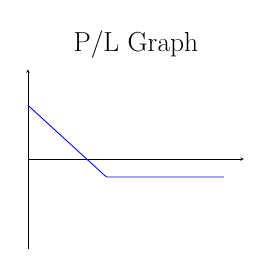
\begin{tikzpicture}[scale=0.4, declare function={func(\x) = (\x <= 2) * (1.5-\x) + (\x > 2) * (-0.5);}]
\begin{axis}[domain=0:5, ymin=-2.5, ymax=2.5, xmax=5.5, axis y line=left, axis x line=middle,
xtick=\empty, ytick=\empty, samples=100, title=\Huge{P/L Graph}]
\addplot[blue, thick]{func(x)}; \end{axis} \end{tikzpicture}
\end{center}

\item We can observe that the payoff graph of the cap can be obtained by
shifting the payoff graph of long put \emph{downward} by \(K\). So, the cap can
also be ``composed'' using a \emph{long put} on \faIcon{apple-alt} and a short
bond.

To be more precise, we can ``decompose'' the payoff graph like below:
\begin{center}
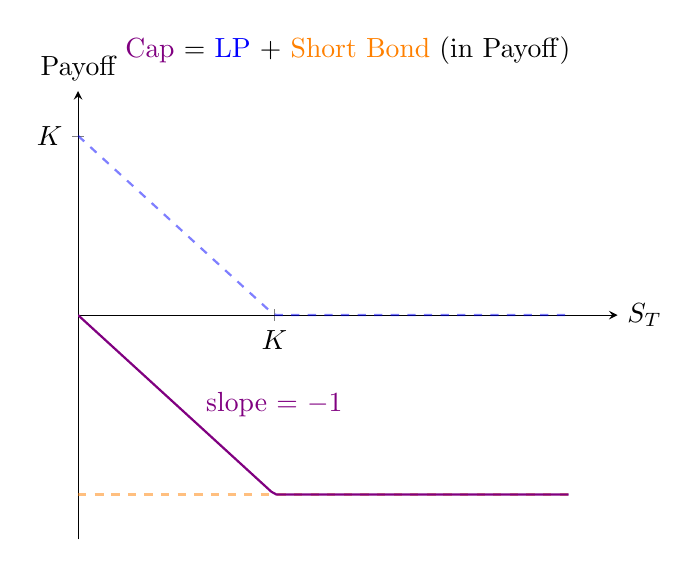
\begin{tikzpicture}[
declare function={
lp(\x) = (\x <= 2) * (2-\x) + (\x > 2) * 0;
sb(\x) = -2;
}
]
\begin{axis}[domain=0:5, ymin=-2.5, ymax=2.5, xmax=5.5, axis y line=left, axis x line=middle,
xtick={2}, title={{\color{violet}Cap} = {\color{blue}LP} + {\color{orange}Short Bond} (in Payoff)},
xticklabel={\(K\)},
ytick={2},
yticklabel={\(K\)}, ylabel=Payoff, ylabel style={at={(axis description cs:0,1)}, anchor=south, rotate=-90},
xlabel=\(S_T\),
xlabel style={anchor=west}, samples=100
]
\addplot[blue, thick, dashed, opacity=0.5]{lp(x)};
\addplot[orange, thick, dashed, opacity=0.5]{sb(x)};
\addplot[violet, thick]{sb(x)+lp(x)};
\node[violet] () at (2,-1) {slope = \(-1\)};
\end{axis}
\end{tikzpicture}
\end{center}
Algebraically we can write
\[
\underbrace{-S_T+(S_T-K)_{+}}_{\text{cap payoff}}
=\underbrace{-K+(K-S_T)_{+}}_{\mathclap{\text{``LP + short bond'' payoff}}},
\]
Since cap and ``LP + short bond'' have the same payoff, their (time-0) prices
must be the same by the law of one price.
\end{enumerate}
\subsection{Covered Calls}
\begin{enumerate}
\item P/L graph of writing a call on \faIcon{apple-alt}:
\begin{center}
\begin{tikzpicture}[declare function={func(\x) = (\x <= 2) * 0.5 + (\x > 2) * -(x-2.5);}]
\begin{axis}[domain=0:5, ymin=-3.5, ymax=1, xmax=5.5, axis y line=left, axis x line=middle,
xtick={2.5}, xticklabels={\(K+C_0e^{rT}\)}, xticklabel style={yshift=0.8cm, xshift=0.8cm},
ytick={0.5}, yticklabels={\(C_0e^{rT}\)}, ylabel=P/L,
ylabel style={at={(axis description cs:0,1)}, anchor=south, rotate=-90},
xlabel=\(S_T\),
xlabel style={anchor=west}, samples=100
]
\addplot[blue, thick]{func(x)};
\node[red] at (3,-1.5) {risk \faIcon{exclamation-triangle}};
\draw[opacity=0.5, red, line width=0.2cm, line cap=round] (2.6,-0.1) -- (5,-2.5);
\end{axis}
\end{tikzpicture}
\end{center}

\item To hedge this risk \faIcon{shield-alt}, we can long \faIcon{apple-alt}
since the ``later positive'' part of the P/L graph for ``long
\faIcon{apple-alt}'' can help reducing the risk:
\begin{center}
\begin{tikzpicture}[]
\begin{axis}[domain=0:5, ymin=-2.5, ymax=2.5, xmax=5.5, axis y line=left, axis x line=middle,
xtick={2.2}, ytick={-2.2}, title={Long \faIcon{apple-alt}},
xticklabel={\(S_0e^{rT}\)}, xticklabel style={xshift=0.3cm},
yticklabel={\(-S_0e^{rT}\)},
ylabel=P/L,
ylabel style={at={(axis description cs:0,1)}, anchor=south, rotate=-90},
xlabel=\(S_T\),
xlabel style={anchor=west}
]
\addplot[blue, thick]{x-2.2};
\draw[opacity=0.5, ForestGreen, line width=0.2cm, line cap=round] (2.3,0.1) -- (5,2.8);
\end{axis}
\end{tikzpicture}
\end{center}
\begin{remark}
\item Of course the P/L graph of LC on \faIcon{apple-alt} also has a ``later
positive'' part. But if we long a call on \faIcon{apple-alt}, we simply close
out the position, which is not so interesting.
\item ``Long forward on \faIcon{apple-alt}'' also has the same P/L graph as
``long \faIcon{apple-alt}'', so long forward is not that much ``different''
from long \faIcon{apple-alt}. Still, we shall consider long \faIcon{apple-alt}
here.
\end{remark}
The act of writing the call \emph{together with} long \faIcon{apple-alt} is
known as \emph{writing}/\emph{selling} a \defn{covered call} (on
\faIcon{apple-alt}). In other words,
\[
\text{short covered call} = \text{short call} + \text{long \faIcon{apple-alt}}.
\]
\begin{note}
In contrast with \emph{writing a covered call} on \faIcon{apple-alt}, the act
of writing a call on \faIcon{apple-alt} without having any position in
\faIcon{apple-alt} simultaneously is known as \emph{writing} a \defn{naked
call} (or \defn{uncovered call}).  (``Naked'' and ``uncovered'' have
``similar'' meaning.)
\end{note}
\item The P/L graph of short covered call is:
\begin{center}
\begin{tikzpicture}[
declare function={
sc(\x) = (\x <= 2) * 0.5 + (\x > 2) * -(\x-2.5);
la(\x) = (\x-2.2);
}
]
\begin{axis}[domain=0:5, ymin=-2.5, ymax=2.5, xmax=5.5, axis y line=left, axis x line=middle,
title={{\color{violet}Short Covered Call} = {\color{blue}SC} + {\color{orange}Long \faIcon{apple-alt}}}, xtick={2.5}, xticklabels={\(K+C_0e^{rT}\)},
ytick={0.5}, yticklabels={\(C_0e^{rT}\)},
ylabel=P/L,
ylabel style={at={(axis description cs:0,1)}, anchor=south, rotate=-90},
xlabel=\(S_T\),
xlabel style={anchor=west}, samples=100
]
\addplot[blue, thick, dashed, opacity=0.5]{sc(x)};
\addplot[orange, thick, dashed, opacity=0.5]{la(x)};
\addplot[violet, thick]{sc(x)+la(x)};
\draw[opacity=0.4, ForestGreen, line width=0.2cm, line cap=round, line join=round] (2.6,0.3) -- (5,0.3);
\draw[-Latex, dashed, ForestGreen] (4,-1.3) to[bend right] (4.5,0.2);
\node[ForestGreen] at (4.5,-0.7) {eliminated risk};
\draw[opacity=0.4, red, line width=0.2cm, line cap=round, line join=round] (0.1,-1.6) -- (1.6,-0.1);
\node[red, text width=2cm] at (1.6,-1.3) {risk \faIcon{exclamation-triangle} (side effect)};
\end{axis}
\end{tikzpicture}
\end{center}
We can note that \emph{another} risk is created as a side effect,
unfortunately. However, as this risk is now ``limited'' (unlike the unlimited
potential loss for SC), the situation may be said to be ``improved''.  (In some
sense, we are ``exchanging'' the risk we face for  another kind of risk.)
\item The P/L of the short covered call is
\[
\underbrace{-(S_T-K)_{+}+C_0e^{rT}}_{\text{SC}}+\underbrace{S_T-S_0e^{rT}}_{\text{long \faIcon{apple-alt}}}
=S_T-(S_T-K)_{+}+(C_0-S_0)e^{rT}.
\]
\item Now, consider its payoff graph:
\begin{center}
\begin{tikzpicture}[
declare function={
sc(\x) = (\x <= 2) * 0 + (\x > 2) * -(\x-2);
la(\x) = (\x);
}
]
\begin{axis}[domain=0:5, ymin=-2.5, ymax=2.5, xmax=5.5, axis y line=left, axis x line=middle,
title={{\color{violet}Short Covered Call} = {\color{blue}SC} + {\color{orange}Long \faIcon{apple-alt}}},
xtick={2}, xticklabels={\(K\)},
ytick=\empty,
ylabel=Payoff,
ylabel style={at={(axis description cs:0,1)}, anchor=south, rotate=-90},
xlabel=\(S_T\),
xlabel style={anchor=west}, samples=100
]
\addplot[blue, thick, dashed, opacity=0.5]{sc(x)};
\addplot[orange, thick, dashed, opacity=0.5]{la(x)};
\addplot[violet, thick]{sc(x)+la(x)};
\end{axis}
\end{tikzpicture}
\end{center}
The ``shape'' of the graph looks like the payoff graph for SP:

\begin{center}
\begin{tikzpicture}[scale=0.6, declare function={func(\x) = (\x <= 2) * -(2-\x) + (\x > 2) * 0;}]
\begin{axis}[domain=0:5, ymin=-2.5, ymax=2.5, xmax=5.5, axis y line=left, axis x line=middle,
xtick=\empty, ytick=\empty, samples=100]
\addplot[blue, thick]{func(x)};
\end{axis}
\end{tikzpicture}
\end{center}

Indeed, short covered call shares the same payoff as ``SP + long bond'' (hence
they have the same price):
\begin{center}
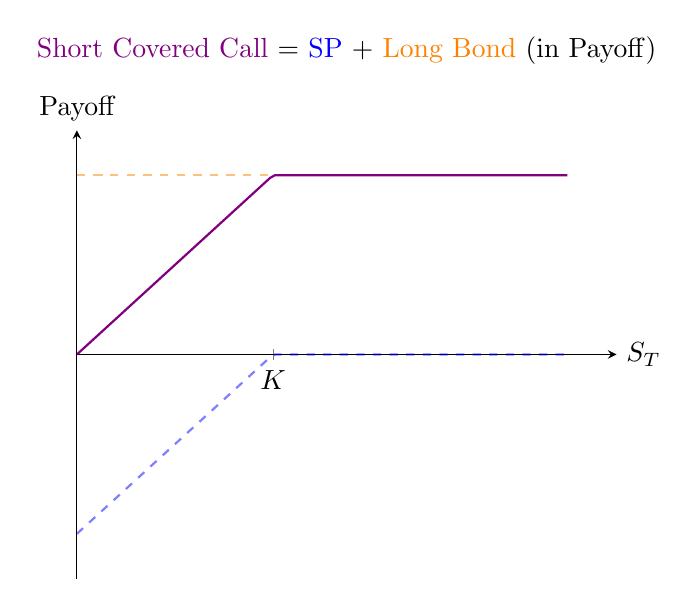
\begin{tikzpicture}[
declare function={
sp(\x) = (\x <= 2) * -(2-x) + (\x > 2) * 0;
lb(\x) = 2;
}
]
\begin{axis}[domain=0:5, ymin=-2.5, ymax=2.5, xmax=5.5, axis y line=left, axis x line=middle,
title={{\color{violet}Short Covered Call} = {\color{blue}SP} + {\color{orange}Long Bond} (in Payoff)},
title style={yshift=0.5cm},
xtick={2}, xticklabels={\(K\)},
ytick=\empty,
ylabel=Payoff,
ylabel style={at={(axis description cs:0,1)}, anchor=south, rotate=-90},
xlabel=\(S_T\),
xlabel style={anchor=west}, samples=100
]
\addplot[blue, thick, dashed, opacity=0.5]{sp(x)};
\addplot[orange, thick, dashed, opacity=0.5]{lb(x)};
\addplot[violet, thick]{sp(x)+lb(x)};
\end{axis}
\end{tikzpicture}
\end{center}
\end{enumerate}

\subsection{Covered Puts}
\begin{enumerate}
\item P/L graph of writing a put on \faIcon{apple-alt}:
\begin{center}
\begin{tikzpicture}[declare function={func(\x) = (\x <= 2) * -(1.5-x) + (\x > 2) * 0.5;}]
\begin{axis}[domain=0:5, ymin=-3.5, ymax=1, xmax=5.5, axis y line=left, axis x line=middle,
xtick={1.5}, xticklabels={\(K-P_0e^{rT}\)}, xticklabel style={yshift=0.8cm, xshift=-0.5cm},
ytick={0.5}, yticklabels={\(P_0e^{rT}\)}, ylabel=P/L,
ylabel style={at={(axis description cs:0,1)}, anchor=south, rotate=-90},
xlabel=\(S_T\),
xlabel style={anchor=west}, samples=100, title=Short Put
]
\addplot[blue, thick]{func(x)};
\draw[opacity=0.4, red, line width=0.2cm, line cap=round, line join=round] (0.1,-1.4) -- (1.4,-0.1);
\node[red] at (1.2,-1) {risk \faIcon{exclamation-triangle}};
\end{axis}
\end{tikzpicture}
\end{center}

\item In a similar manner, to hedge this risk \faIcon{shield-alt}, we can short
\faIcon{apple-alt} since the ``initial positive'' part of the P/L graph for
``short \faIcon{apple-alt}'' can help reducing the risk:
\begin{center}
\begin{tikzpicture}[]
\begin{axis}[domain=0:5, ymin=-2.5, ymax=2.5, xmax=5.5, axis y line=left, axis x line=middle,
xtick={2.2}, ytick={2.2}, title={Short \faIcon{apple-alt}},
xticklabel={\(S_0e^{rT}\)}, xticklabel style={xshift=-0.3cm},
yticklabel={\(S_0e^{rT}\)},
ylabel=P/L,
ylabel style={at={(axis description cs:0,1)}, anchor=south, rotate=-90},
xlabel=\(S_T\),
xlabel style={anchor=west}
]
\addplot[blue, thick]{2.2-x};
\draw[opacity=0.5, ForestGreen, line width=0.2cm, line cap=round] (0.1,2.1) -- (2.1,0.1);
\end{axis}
\end{tikzpicture}
\end{center}
Likewise, \emph{writing} a \defn{covered put} (on \faIcon{apple-alt}) means
writing a put on \faIcon{apple-alt} together with short \faIcon{apple-alt},
i.e.,
\[
\text{short covered put} = \text{short put} + \text{short \faIcon{apple-alt}}.
\]
\begin{note}
In contrast with \emph{writing a covered put} on \faIcon{apple-alt}, the act of
writing a put on \faIcon{apple-alt} without having any position in
\faIcon{apple-alt} simultaneously is known as \emph{writing} a \defn{naked put}
(or \defn{uncovered put}).
\end{note}
\item The P/L graph of short covered put is:
\begin{center}
\begin{tikzpicture}[
declare function={
sp(\x) = (\x <= 2) * -(1.5-\x) + (\x > 2) * 0.5;
sa(\x) = (2.2-\x);
}
]
\begin{axis}[domain=0:5, ymin=-2.5, ymax=2.5, xmax=5.5, axis y line=left, axis x line=middle,
title={{\color{violet}Short Covered Put} = {\color{blue}SP} + {\color{orange}Short \faIcon{apple-alt}}},
xtick={1.5}, xticklabels={\(K-P_0e^{rT}\)}, xticklabel style={yshift=0.7cm},
ytick={0.5}, yticklabels={\(P_0e^{rT}\)},
ylabel=P/L,
ylabel style={at={(axis description cs:0,1)}, anchor=south, rotate=-90},
xlabel=\(S_T\),
xlabel style={anchor=west}, samples=100
]
\addplot[blue, thick, dashed, opacity=0.5]{sp(x)};
\addplot[orange, thick, dashed, opacity=0.5]{sa(x)};
\addplot[violet, thick]{sp(x)+sa(x)};
\draw[opacity=0.4, ForestGreen, line width=0.2cm, line cap=round, line join=round] (0.1,0.7) -- (1.9,0.7);
\draw[-Latex, dashed, ForestGreen] (0.7,-0.7) to[bend left] (0.9,0.6);
\node[ForestGreen] at (0.6,-0.3) {elim.\ risk};
\draw[opacity=0.4, red, line width=0.2cm, line cap=round, line join=round] (2.8,-0.1) -- (5,-2.3);
\node[red] at (2.3,-1.3) {risk \faIcon{exclamation-triangle} (side effect)};
\end{axis}
\end{tikzpicture}
\end{center}
Since the risk in fact changes from \emph{limited} (SP) to \emph{unlimited}
(here), the situation may be seen as ``worsened'' unfortunately. Thus, we
seldom write covered put in practice.

\item Now, consider its payoff graph:
\begin{center}
\begin{tikzpicture}[
declare function={
sp(\x) = (\x <= 2) * -(2-\x) + (\x > 2) * 0;
sa(\x) = (-\x);
}
]
\begin{axis}[domain=0:5, ymax=2.5, xmax=5.5, axis y line=left, axis x line=middle,
title={{\color{violet}Short Covered Put} = {\color{blue}SP} + {\color{orange}Short \faIcon{apple-alt}}},
xtick={2}, xticklabels={\(K\)}, xticklabel style={yshift=0.7cm},
ytick=\empty,
ylabel=Payoff,
ylabel style={at={(axis description cs:0,1)}, anchor=south, rotate=-90},
xlabel=\(S_T\),
xlabel style={anchor=west}, samples=100
]
\addplot[blue, thick, dashed, opacity=0.5]{sp(x)};
\addplot[orange, thick, dashed, opacity=0.5]{sa(x)};
\addplot[violet, thick]{sp(x)+sa(x)};
\end{axis}
\end{tikzpicture}
\end{center}
The ``shape'' of the graph looks like the payoff graph for SC:

\begin{center}
\begin{tikzpicture}[scale=0.6, declare function={func(\x) = (\x <= 2) * 0 + (\x > 2) * -(\x-2);}]
\begin{axis}[domain=0:5, ymin=-2.5, ymax=2.5, xmax=5.5, axis y line=left, axis x line=middle,
xtick=\empty, ytick=\empty, samples=100]
\addplot[blue, thick]{func(x)};
\end{axis}
\end{tikzpicture}
\end{center}

Similarly, we can note that short covered call has the same payoff as ``SC +
short bond'' (so they have the same price):
\begin{center}
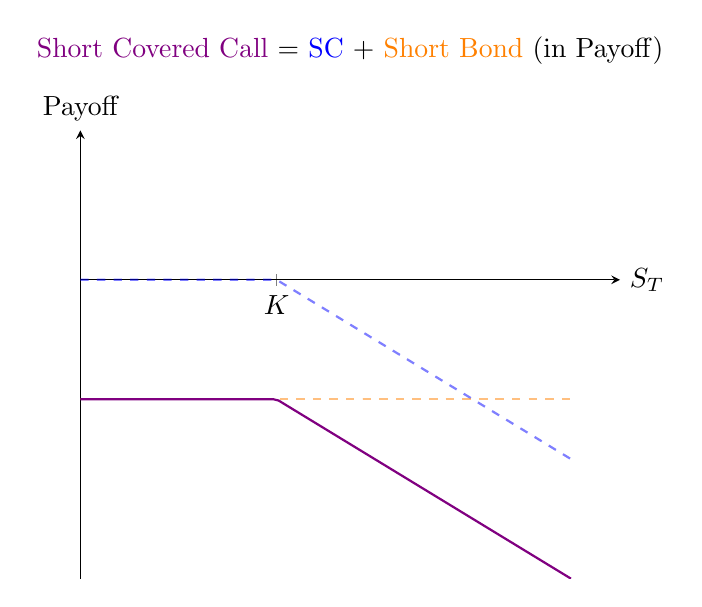
\begin{tikzpicture}[
declare function={
sc(\x) = (\x <= 2) * 0 + (\x > 2) * -(x-2);
sb(\x) = -2;
}
]
\begin{axis}[domain=0:5, ymax=2.5, xmax=5.5, axis y line=left, axis x line=middle,
title={{\color{violet}Short Covered Call} = {\color{blue}SC} + {\color{orange}Short Bond} (in Payoff)},
title style={yshift=0.5cm},
xtick={2}, xticklabels={\(K\)},
ytick=\empty,
ylabel=Payoff,
ylabel style={at={(axis description cs:0,1)}, anchor=south, rotate=-90},
xlabel=\(S_T\),
xlabel style={anchor=west}, samples=100
]
\addplot[blue, thick, dashed, opacity=0.5]{sc(x)};
\addplot[orange, thick, dashed, opacity=0.5]{sb(x)};
\addplot[violet, thick]{sc(x)+sb(x)};
\end{axis}
\end{tikzpicture}
\end{center}
\end{enumerate}
\subsection{Synthetic Forward}
\subsection{Put-Call Parity}
\label{subsect:put-call-parity}
